\documentclass{article}

\usepackage{authblk}
\usepackage{amsmath}
\usepackage{tikz}
\usepackage{chngcntr}
\usepackage{caption}
\usepackage{subcaption}
\usepackage{lipsum}
\usepackage{minted}
\usepackage{graphicx}

\graphicspath{ {./} }

\usepackage{titlesec}

\makeatletter
\newcommand{\setappendix}{Appendix~\thesection:~}
\newcommand{\setsection}{\thesection~}
\titleformat{\section}{\bfseries\LARGE}{%
  \ifnum\pdfstrcmp{\@currenvir}{appendices}=0
    \setappendix
  \else
    \setsection
  \fi}{0em}{}
\makeatother

\usepackage[titletoc]{appendix}

\counterwithin{figure}{section}

\author{Aurora Zuoris \\ \normalsize{aurora.zuoris101@alu.ulpgc.es}}
\affil{Universidad de Las Palmas de Gran Canaria}
\title{Matrix multiplication at the speed of light}

\begin{document}

\maketitle

\abstract{
This paper will discuss various methods for implementing matrix multiplication,
along with their advantages and disadvantages for different situations.
Languages explored are Python, Java, C, Rust, and SQL, with methods including
naive, improving cache hits, parallelization, vectoring and trying to leverage the GPU.
}

\section{Introduction}

Matrix multiplication is becoming increasingly important in the modern world.
Two big examples are machine learning and graph theory, both of which are
becoming more and more important with the rise of big data.
Thus knowing what the best ways to implement matrix multiplication in
various situations is crucial for the future of computing.

In this paper, we will explore various ways to speed up matrix multiplication.
One major use for matrix multiplication in the past decade is in deep machine learning,
as they are used to represent the weights and biases of neural networks, such that
a forward pass can be done by multiplying the input by the weight matrix and adding the bias vector,
limiting the speed of the forward pass to the speed of matrix multiplication.

\section{Methotology}

The matrix multiplication algorithms will be implemented in various languages, using a plethora
of different optimization techniques, and then benchmarked to see which is the fastest using each
language's timing libraries to get the most accurate results possible.

For brevity and because of time constraints, not all possible combinations of languages and optimization
techniques will be explored, but rather a subset of the most interesting ones.

\subsection{Python}

To start with, python will be used as a baseline, as it is commonly used in machine learning and it's known to be slow.
So it will be interesting to see how much of a difference there is between python and other languages.

The python implementation consists of a class with a field for the matrix, and a method for multiplying two matrices.
The multiplication is implemented using list comprehension, which is more pythonic than using for loops, and can be faster too
given that they use more optimized code under the hood. Making it a more fair comparison to other languages.

The code used is as follows:

\begin{minted}[tabsize=2,]{python}
@dataclass
class matrix:
	buff: list[list[float]]

	# constructors ommited for brevity ...
	
	def __matmul__(self, other):
		if len(self.buff[0]) != len(other.buff):
			raise ValueError("Matrix dimensions do not match")
		return matrix([
			[
				sum(a * b for a, b in zip(row, col))
				for col
				in zip(*other.buff)
			]
			for row
			in self.buff
		])
\end{minted}

For the benchmarking, the code is as follows:

\begin{minted}[tabsize=2]{python}
results = defaultdict(list)

for n in range(1, 13):
	size = 2 ** n
	a = matrix.random(size)
	b = matrix.random(size)

	start = time()
	c = a @ b
	end = time()

	results['size'].append(size)
	results['time'].append(end - start)

results = pd.DataFrame(results)
\end{minted}

\subsection{Java}

Java is a language that is commonly used in industry, and it's known to be faster than python.
The implementation is similar to the python one, with a class for the matrix and a method for multiplying two matrices.
The multiplication is implemented using for loops, as they are the most common way to do it in java.
For the matrix itself, it is implemented with a 1D array, storing the matrix in row-major order.
This is done as it's unnecessary to do $N+1$ allocations for a matrix of size $N\times N$,
when it can be done with just one allocation. Aditionally, being explicit about the order of the matrix in memory
is a good way to improve cache hits, as will be seen later, and also leads to better self documentation.

The implementation is as follows:

\begin{minted}[tabsize=2]{java}
public class Matrix {
	private float data[];
	private int size;

	public Matrix(int size) {
		this.size = size;
		this.data = new float[size * size];
	}

	// other constructors ommited for brevity ...

	public float get(int row, int column) {
		return data[row * size + column];
	}

	public void set(int row, int column, float value) {
		data[row * size + column] = value;
	}

	public Matrix multiply(Matrix other) {
		if (size != other.size) {
			throw new IllegalArgumentException("Matrix dimensions do not match");
		}
		Matrix result = new Matrix(size);
		for (int row = 0; row < size; row++) {
			for (int column = 0; column < size; column++) {
				float sum = 0;
				for (int k = 0; k < size; k++) {
					sum += get(row, k) * other.get(k, column);
				}
				result.set(row, column, sum);
			}
		}
		return result;
	}
}

\end{minted}

This is benchmarked using the following code:

\begin{minted}[tabsize=2]{java}
Random random = new Random();

for (int i = 1; i <= 12; i++) {
	int n = (1 << i);
	Matrix a = new Matrix(n, random);
	Matrix b = new Matrix(n, random);

	long start = System.nanoTime();
	Matrix c = a.multiply(b);
	long end = System.nanoTime();
	System.out.println("Size: " + n + " | Time: "
		+ String.format("%.6f", (end - start) * 1e-9 ));
}
\end{minted}

\subsection{C}

For C, we will first do a naive implementation, and then we will try to improve it.
The naive implementation is similar to the java one, an allocation in row-major order, and then a function that simply does a nested for loop.
It is also worth noting that in C, it'll also be important what optimization flags are used when compiling, as they can make a big difference.

The implementation is as follows:

\begin{minted}[tabsize=2]{c}
void matmul(float *out, float *a, float *b, size_t size)
{
	for (size_t row = 0; row < size; row++)
	{
		for (size_t col = 0; col < size; col++)
		{
			float s = 0;
			for (size_t k = 0; k < size; k++)
			{
				s += a[k + row * size] * b[col + k * size];
			}
			out[col + row * size] = s;
		}
	}
}
\end{minted}

\newpage

The benchmarking code is as follows:

\begin{minted}[tabsize=2]{c}
printf("Size,Time\n");
fflush(stdout);
int n = 1;
for(int i = 1; i <= sizes; i++) {
	n *= 2;
	struct stopwatch sw;
	float *A = malloc(n * n * sizeof(float));
	float *B = malloc(n * n * sizeof(float));
	float *C = malloc(n * n * sizeof(float));
	for (int i = 0; i < n; i++)
	{
		for (int j = 0; j < n; j++)
		{
			A[i + j * n] = rand() / RAND_MAX;
			B[i + j * n] = rand() / RAND_MAX;
		}
	}

	stopwatch_start(&sw);
	matmul(C, A, B, n);
	stopwatch_stop(&sw);

	asm volatile("": : "g"(C) : "memory");

	double duration = stopwatch_elapsed(&sw);

	printf("%d,%f\n", n, duration);
	fflush(stdout);
}
\end{minted}

\subsection{C with cache locality}

The first improvement we will try to do is to improve cache hits.

One way to improve the speed of matrix multiplication is to try to improve cache hits.
This can be done by having the second matrix be looped by rows in the inner loop.
While this does not correspond to an actual matrix multiplication, as the second matrix is looped trough incorrectly, it does
correspond to $AB^\top$. To fix this discrepancy, one needs to first do a transpose on the second vector.
While this is extra computation that needs to be done, a transposition is $O(n^2)$ in time complexity, while the multiplication
is $O(n^3)$, so while it may seem like it would slow it down, you can think of this addition as procuring $O(n^2)$ work to have
$O(n^3)$ computations be up to $200$ times faster, or however much faster it is to fetch data from the cache rather than the RAM.
This can be visualized in figure \ref{fig:cache}.


\begin{figure}[h!]
	\begin{subfigure}{0.3\textwidth}
		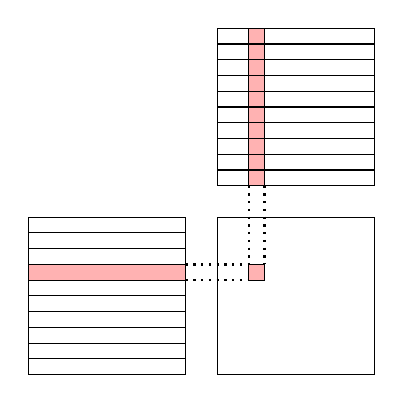
\begin{tikzpicture}[scale=0.2]
			\draw (0,0) rectangle +(10,10);
			\foreach \y in {1, ..., 9}
			{
				\draw (0, \y) -- (10, \y);
			}
			\filldraw[fill=red!30!white] (0, 6) rectangle +(10, 1);
			\draw (12,0) rectangle +(10, 10);
			\draw (12, 12) rectangle +(10, 10);
			\filldraw[fill=red!30!white] (14, 12) rectangle +(1, 10);
			\foreach \y in {1, ..., 9}
			{
				\draw (12, 12+\y) -- +(10, 0);
			}
			\draw[dotted, thick]
				(10, 6) -- (14, 6)
				(10, 7) -- (14, 7)
				(14, 12) -- (14, 7)
				(15, 12) -- (15, 7)
				;
			\draw[fill=red!30!white] (14, 6) rectangle +(1, 1);
		\end{tikzpicture}
	\caption{
		naive multiplication has a lot of cache misses
	}
	\end{subfigure}
	\hfill
	\begin{subfigure}{0.3\textwidth}
		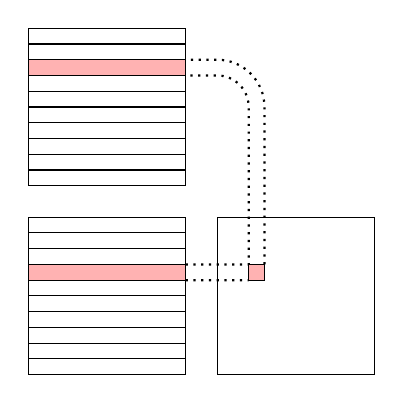
\begin{tikzpicture}[scale=0.2]
			\draw (0,0) rectangle +(10,10);
			\filldraw[fill=red!30!white] (0, 6) rectangle +(10, 1);
			\foreach \y in {1, ..., 9}
			{
				\draw (0, \y) -- (10, \y);
			}
			\draw (12,0) rectangle +(10, 10);
			\draw (0, 12) rectangle +(10, 10);
			\filldraw[fill=red!30!white] (0, 12+7) rectangle +(10, 1);
			\foreach \y in {1, ..., 9}
			{
				\draw (0, 12+\y) -- +(10, 0);
			}
			\draw[dotted, thick]
				(10, 6) -- (14, 6)
				(10, 7) -- (14, 7) -- (14, 17) arc[start angle=0, end angle=90, radius=2] -- (10, 12+7)
				(15, 7) -- (15, 17) arc[start angle=0, end angle=90, radius=3] -- (10, 12+8)
				;
			\draw[fill=red!30!white] (14, 6) rectangle +(1, 1);
		\end{tikzpicture}
	\caption{
		$AB^\top$ has more cache hits
	}
	\end{subfigure}
	\caption{Matrix multiplication cache hit optimization}
	\label{fig:cache}
\end{figure}

\newpage

The code for the multiplication is as follows:

\begin{minted}[tabsize=2]{c}
void matmul(float *out, float *a, float *b, size_t size)
{
	for (size_t row = 0; row < size; row++)
	{
		for (size_t col = 0; col < size; col++)
		{
			float s = 0;
			for (size_t k = 0; k < size; k++)
			{
				s += a[k + row * size] + b[k + col * size];
			}
			out[col + row * size] = s;
		}
	}
}
\end{minted}

It should be noted that this is almost identical to the naive implementation,
only changing the indexing of the second matrix.
One way to see that this is more cache friendly is to look at the indexing of the inner most loop,
they're both accessing \mintinline{c}{[k + row * size]} and \mintinline{c}{[k + col * size]},
as k is the variable of the inner most loop, then each iteration will be accessing very close memory locations.
Unlike in the naive implementation, which used \mintinline{c}{[col + k * size]} for the second one,
where k is still the variable of the inner most loop, but it is multiplied by size, so each iteration will be accessing
memory locations that are far apart, leading to more cache misses.

Altough with this implementation, it's not directly matrix multiplication, $AB$,
but rather $AB^\top$, as the second matrix is looped trough by rows instead of by columns.
Thus to fix this, one needs to first transpose the second matrix, and then do the multiplication.
The matrix transposition implementation is as follows:

\begin{minted}[tabsize=2]{c}
void transpose(float *mat, size_t size)
{
	for (size_t i = 0; i < size; i++)
	{
		for (size_t j = 0; j < i; j++)
		{
			float tmp = mat[i + j * size];
			mat[i + j * size] = mat[j + i * size];
			mat[j + i * size] = tmp;
		}
	}
}
\end{minted}

The benchmarking code is similar to the naive implementation, with the only addition being that
a transpose is done before the multiplication, thus replacing the timing section with this:

\begin{minted}[tabsize=2]{c}
stopwatch_start(&sw);
transpose(B, n);
matmul(C, A, B, n);
stopwatch_stop(&sw);
\end{minted}

\subsection{C with parallelization}

Finally for C, the most optimized version will be implemented, attempting to use both parallelization and vectorization.
This implementation uses pthreads to parallelize the multiplication, and SIMD intrinsics to vectorize it.
This is done by splitting the elements of the matrix into chunks, and then having each thread calculate the result for all the elements in its chunk.
As the chunks are independent, and the two input matrices are only ever read, this is a safe operation to do in parallel without any need for synchronization other than joining
the threads at the end.

The code is split across 2 functions and a struct,
one function for dispaching the tasks to the threads, the struct which holds what tasks each thread should do,
and the function that each thread runs, which is a more optimized version of the cache multiplication with SIMD, but only for a subset of the matrix.

\newpage

The struct and code for dispatching the tasks is as follows:

\begin{minted}[tabsize=2]{c}
struct matmul_job
{
	size_t size, start_idx, len;
	float *left, *right, *result;
};

void matmul(float *out, float *a, float *b, size_t size)
{
	struct matmul_job tasks[N_THREADS];
	pthread_t threads[N_THREADS - 1];
	size_t tasks_per_thread = size * size / N_THREADS;
	size_t leftover_tasks = size * size % N_THREADS;

	for (size_t i = 0; i < N_THREADS; i++)
	{
		tasks[i].size = size;
		tasks[i].left = a;
		tasks[i].right = b;
		tasks[i].result = out;
		tasks[i].start_idx = i * tasks_per_thread
			+ (i < leftover_tasks ? i : leftover_tasks);
		tasks[i].len = size * size / N_THREADS + (i < leftover_tasks ? 1 : 0);
		if (i < N_THREADS - 1)
		{
			pthread_create(&threads[i], NULL, matmul_task, &tasks[i]);
		}
		else
		{
			matmul_task(&tasks[i]);
		}
	}
	for (int i = 0; i < N_THREADS - 1; i++)
	{
		pthread_join(threads[i], NULL);
	}
}
\end{minted}

\newpage

While the code for the task that each thread runs is as follows:

\begin{minted}[tabsize=2]{c}
void *matmul_task(void *ptr)
{
	struct matmul_job *job = (struct matmul_job *)ptr;
	size_t size = job->size;
	size_t start_idx = job->start_idx;
	size_t len = job->len;
	float *left = job->left;
	float *right = job->right;
	float *result = job->result;

	for (size_t idx = start_idx; idx < (start_idx + len); idx++)
	{
		size_t row = idx / size;
		size_t col = idx % size;
		float s = 0;
		size_t k = 0;
		if (size >= 4)
			for (; k < size - 3; k += 4)
			{
				float simd_res[4];
				__m128 l, r, prod;
				l = _mm_load_ps(&left[k + row * size]);
				r = _mm_load_ps(&right[k + col * size]);
				prod = _mm_mul_ps(l, r);
				_mm_store_ps(simd_res, prod);
				s += simd_res[0] + simd_res[1] + simd_res[2] + simd_res[3];
			}
		for (; k < size; k++)
		{
			s += left[k + row * size] * right[k + col * size];
		}
		result[col + row * size] = s;
	}
	return NULL;
}
\end{minted}

The benchmarking is done exactly the same as in the last section.

\subsection{Rust with GPU}

Last but not least, we will try to leverage the GPU to speed up matrix multiplication.
For this, we will use the rust programming language, as it has a good, modern library for GPU programming called wgpu.

WGPU is based on the WebGPU standard, which is a new standard for GPU programming meant to target the web and replace WebGL.
It may seem strange to use a web standard for GPU programming, but it is actually a good idea, as modern web standards are designed to be
highly portable and as fast as native applications, meaning that using modern web standards will lead to programs that are as fast as native ones,
and can be run on any platform, from desktops to mobile phones, to even web browsers.
It is notable to say that even if it is a web standard, one can still use it to make native applications, as it is not tied to the web in any way
other than its origins.

This leads to a very portable and fast library that can leverage the GPU, unlike most other libraries that use the GPU which
are usually tied to a specific platform, such as CUDA, which is only available on Nvidia GPUs and only on desktops, which also need meticulous setup
to get working correctly. WebGPU on the other hand, compiles to SPIR-V, which is a standard intermediate representation for shaders, which can then be
compiled to native code for any platform, and can be run on any platform that supports Vulkan, DirectX 12, Metal, or OpenGL, which is almost all of them.
Leading to a very simple, batteries included library that can be used to leverage the GPU for any platform.

A notable trivia about the specific library used here, wgpu, is that it's one of the two main implementations of WebGPU, being used in the Firefox browser to implement WebGPU.
The other implementation being Dawn, written in C++, which is used in Chromium browsers to implement WebGPU.

Unlike other implementations, this one is much more convoluted, as it is not as simple as just calling a function to do matrix multiplication,
but rather it needs to be done in a shader, which is a program that runs on the GPU, and is written in a special language called WGSL.
And thus there also is lots of boilerplate code to set up the GPU, and to pass the matrices to the shader, and to get the result back.
To get a full explanation of how this works, see appendix \ref{sec:wgpu}.
But the basic gist of it can be found in the WGSL code, which is as follows:

\newpage

\begin{minted}[tabsize=2]{wgsl}
 @group(0)
 @binding(0)
 var<uniform> size: u32;

 @group(0)
 @binding(1)
 var<storage, read_write> mat_out: array<f32>;

 @group(1)
 @binding(1)
 var<storage, read_write> mat_left: array<f32>;

 @group(2)
 @binding(1)
 var<storage, read_write> mat_right: array<f32>;

@compute @workgroup_size(16, 16)
fn compute(@builtin(global_invocation_id) gid: vec3<u32>)
{
	let x = gid.x;
	let y = gid.y;
	if (x >= size || y >= size)
	{
		return;
	}
	var sum = 0.0;
	for (var k = 0u; k < size; k++)
	{
		let a = mat_left[y * size + k];
		let b = mat_right[k * size + x];
		sum += a * b;
	}
	mat_out[y * size + x] = sum;
}
\end{minted}

This also has implications when it comes to benchmarking, as one could either just measure the time it takes to do the computations on the GPU,
or also include the time it takes to move the data to and from the GPU, which is a much more expensive operation than the actual computation.
For this paper, we will only measure the time it takes to do the computation on the GPU, as that is the only part that is actually done on the GPU.
Altough there is still some overhead included with this method,
as each multiplication will need to have its own compute pass.
In theory it should be possible to stuff multiple multiplications into a single compute pass,
leading to a lower time per multiplication, but this is not done here.

\newpage

As for the benchmarking, it is done using the following code:

\begin{minted}[tabsize=2]{rust}
let gpu = Arc::new(pollster::block_on(Gpu::new()));

let mut rng = rand::thread_rng();

let max_size = 5792;

let mat1 = Matrix::generate(Arc::clone(&gpu), max_size, |_, _| rng.gen());
let mat2 = Matrix::generate(Arc::clone(&gpu), max_size, |_, _| rng.gen());

println!("Size,Time");
let sizes = 12;
for size in (1..=sizes).map(|n| (2u32).pow(n) as usize) {
	let mut left = Matrix::generate(
		Arc::clone(&gpu),
		size,
		|col, row| mat1[(col, row)]
	);
	let mut right = Matrix::generate(
		Arc::clone(&gpu),
		size,
		|col, row| mat2[(col, row)]
	);

	left.move_to_gpu();
	right.move_to_gpu();

	let start = std::time::Instant::now();
	let _ = &left * &right;
	let end = std::time::Instant::now();

	println!("{},{}", size, (end - start).as_secs_f64());
	std::thread::sleep(std::time::Duration::from_millis(700));
}
\end{minted}

It should be noted that
there is some sleeps in the benchmarking code, as the GPU is asynchronous,
and thus there is some synchronization that needs to be done.
This code could be further optimized by making it more asynchronous.

\section{Results and conclusions}

The results of the benchmarks can be seen in figure \ref{fig:results}.
This graph was generated using matplotlib, with the data being generated
using each program's timing libraries and or methods.
Due to the large difference in speed between the different methods,
the graph is in log scale, to better show the differences between the methods.
Aditionally, the x axis, the size of the matrices, is also in log scale,
to further show the differences between the methods when it comes to
small matrices and large matrices.

\begin{figure}[h!]
	\centering
	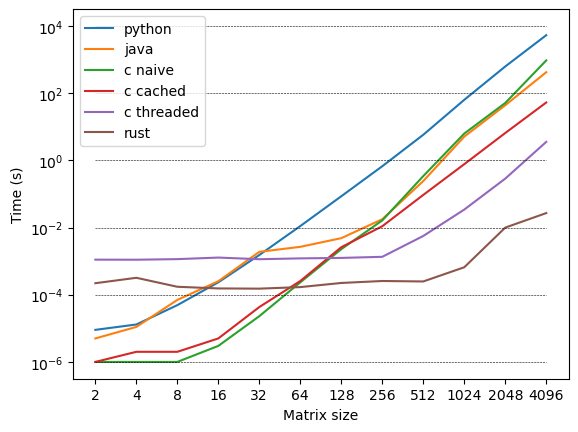
\includegraphics[width=0.8\textwidth]{results.png}
	\caption{Matrix multiplication benchmark results}
	\label{fig:results}
\end{figure}

As can be seen in the graph, the naive python implementation is by far the slowest,
taking over an hour to multiply two $4096\times 4096$ matrices.
Next up, the java implementation starts off just as slow as the python one,
but for the bigger matrices it starts to get faster, getting as fast
as the naive C implementation. This could be due to the JVM's dynamic optimization behavior.
The naive and cache optimized implementations start off just as fast, with the naive
one being marginally faster, until the cache optimized version becomes much faster
for larger matrices.
This could be due to the added overhead in performing the transposes.
For the parallelized version, it can be seen that it has
major overhead for small matrices, having a constant time in the order of magnitude of just under a millisecond,
while the other ones are in the order of microseconds, around 1000 times slower.
But it manages to continue this constant time for much larger matrices, until it grows
just as fast as the other ones, but with a couple orders of magnitude faster.
Finally, the rust WGPU implementation takes this to the extreme, having a similar
overhead but much slower, and managing to keep it constant for larger matrices,
starting to grow with even a few more orders of magnitude faster than the parallelized C implementation,
to the point that what took python over an hour, takes rust just a few milliseconds.

It should be noted that the last two methods depends a lot more on
the hardware used, as the C parallelized method is explicit about
threadding, not something available in all environments, and it also uses
specific SSE intrinsics, which are only available on x86 CPUs.
The rust WGPU implementation is similarly hardware dependent,
as it takes advantage of the GPU.
But this is to be expected, as to have such a large speedup,
one needs to use all the available techniques and hardware at their disposal,
but this leads to less portable and more specific code.

In conclusion, when it comes to implementing matrix multiplication,
a python implementation is not recommended, as it is unaffordably slow.
Altough it should be noted that it is possible to create python libraries
that use C or C++ under the hood, which would be much faster while still
using pyhton for all the more high level code for prototyping and such.
It's just that the low level hot loops should not be implemented in python,
this is one of the reasons that python has a reputation for being a glue language,
as it is very good at calling other languages, but not so good at implementing
performant code itself.
When it comes to java, it is a good language for implementing matrix multiplication,
becoming as fast as C for large matrices. Given that it is a widely used language,
this could lead to it being an acceptable choise for various applications that
are written in Java. It should be noted that it could be further improved, for example
trough the use of cache optimization, while still keeping it portable enough as to not
depend on specific hardware.
When it comes to C, it is a good language for implementing matrix multiplication,
knowing that it is known to be highly portable, and it is also known to be fast,
it is a good choise for implementing matrix multiplication for almost any application,
altough it should be considered that C itself is not a great choice for
prototyping or fast iterations as it is a low level language, and thus it should be
considered to use it with higher level languages that do all the business level
logic that can call into C for the hot loops.
Finally, when it comes to rust and the GPU,
it beats everything else by a large margin, thus it should be the go to choise for
anything that needs to do lots of large matrix multiplications, for example in
deep learning. Altough it should be noted that it is not that great
for much smaller matrices, something very common used for example in graphics
programming.
Thus for that, it would be better to either do it in the CPU,
or use a completely different approach, such as using the GPU's matrix naive types that can support up to 4 by 4 matrices naively.
It should be noted that for most modern deep learning applications,
something similar to the rust WGPU implementation is used,
using libraries such as tensorflow or pytorch, which use CUDA
to leverage the GPU, but this is not as portable as the rust WGPU implementation,
as it is specific to Nvidia GPUs, and it thus does not
bother to be as portable, especially compard to WebGPU, which is designed to be as portable as possible.

\section{Future Work}

There is still lots of room for improvement, especially depending on the use case.
One major one would be to look into the multiplication of sparce matrices,
as that can be very common for graph related tasks.
This is because graphs are usually sparce, most people only have a few friends, not everyone is friends with everyone.
Thus a sparce matrix would represent this better, only storing the connections that exist, and not the ones that don't.
And thus it would be interesting to see how to not only leverage this to speed up matrix multiplication,
but also see how far it can be taken, as it would allow for much larger matrices to be used that would be impossible to use otherwise.

When it comes to further improving dense matrix multiplication as discussed in this paper,
one could look into using some of the techniques discussed here in combination with each other,
such as implementing the cache locality or GPU methods in Java, or Python.
Aditionally, in the last method, using WebGPU with rust,
one could try to further develop it to be able to do multiple multiplications in a single compute pass.
Aditionally, there's still lots of room for improvement in the GPU method, starting with converting
the code to be asynchronous, as this would lead to better synchronization between the CPU and GPU,
as it is interesting to note that bringing in the GPU into this
turns the problem from a CPU bound one to an IO bound one,
as the CPU simply dispatches the task to the GPU, and then waits for it to finish.
Aditionally, there are a bunch of other techniques not explored,
such as the use of Fortran, which is known to be very fast and specifically
designed for scientific computing, which this would be a perfect use case for.
It would also be interesting to compare the speed of the current GPU
method implemented trough WebGPU APIs to that of CUDA, as CUDA is 
the current industry standard for GPU compute programming, especially 
in applications such as deep learning, and thus it would be interesting
to see how it compares to the more portable WebGPU implementation.

\begin{appendices}

\appendix

\section{Implementing matrix multiplication in Wgpu}

\label{sec:wgpu}

Firstly, to use the GPU, there is a lot of bookkeeping that needs to be done,
it is important to realize that the GPU is its own completely different entity,
it has its own memory, its own CPU, its own everything.
Thus to use the GPU, it is akin to managing and controlling the data
of a completely different computer.
To do this, a GPU context struct is created, which holds all the data needed to interact with the GPU,
such as the device, the queue and the compute shaders.

\begin{minted}[tabsize=2]{rust}
pub struct Gpu {
	instance: wgpu::Instance,
	adapter: wgpu::Adapter,
	device: wgpu::Device,
	queue: wgpu::Queue,
	shader: wgpu::ShaderModule,
	pipeline_layout: wgpu::PipelineLayout,
	pipeline: wgpu::ComputePipeline,
	matrix_layout: wgpu::BindGroupLayout,
}
\end{minted}

For initializing this, there is lots of boilerplate code that needs to be done:

\begin{minted}[tabsize=2]{rust}
pub async fn new() -> Gpu {
	let instance = wgpu::Instance::new(Default::default());
	let adapter = instance.request_adapter(&Default::default()).await.unwrap();
	let features = adapter.features();

	let (device, queue) = adapter
		.request_device(
			&wgpu::DeviceDescriptor {
				label: None,
				features,
				limits: Default::default(),
			},
			None,
		)
		.await
		.unwrap();
	let matrix_layout = mat_layout(&device);
	let shader = device.create_shader_module(wgpu::ShaderModuleDescriptor {
		label: Some("matrix multiplication shader"),
		source: wgpu::ShaderSource::Wgsl(include_str!("matmul.wgsl").into()),
	});

	let pipeline_layout = device.create_pipeline_layout(&wgpu::PipelineLayoutDescriptor {
		label: Some("matrix multiplication pipeline layout"),
		bind_group_layouts: &[&matrix_layout, &matrix_layout, &matrix_layout],
		push_constant_ranges: &[],
	});

	let pipeline = device.create_compute_pipeline(&wgpu::ComputePipelineDescriptor {
		label: Some("matrix multiplication pipeline"),
		layout: Some(&pipeline_layout),
		module: &shader,
		entry_point: "compute",
	});

	Gpu {
		instance,
		adapter,
		device,
		queue,
		shader,
		pipeline_layout,
		pipeline,
		matrix_layout,
	}
}
\end{minted}

Next up, for the matrices, there is a struct that holds the data of the matrix,
as the GPU is its own entity, the matrices also need to do
their own bookkeeping, tracking whenever it is the CPU or the GPU which
has the up to date data, and also tracking the GPU buffer that holds the data.
For the sake of ease, each matrix has a reference to the GPU context trough
a shared pointer.

\begin{minted}[tabsize=2]{rust}
#[derive(Copy, Clone, Debug, PartialEq, Eq)]
pub enum Dirty {
	/// The CPU and GPU buffers are in sync.
	Clean,
	/// the GPU buffer has changes not reflected in the CPU buffer.
	CPUDirty,
	/// the CPU buffer has changes not reflected in the GPU buffer.
	GPUDirty,
}

struct MatrixGPUFrame {
	buffer: wgpu::Buffer,
	size_buffer: wgpu::Buffer,
	bind_group: wgpu::BindGroup,
	dirty: Dirty,
}

pub struct Matrix {
	size: usize,
	data: Vec<f32>,
	gpu: Arc<Gpu>,
	gpu_frame: Option<MatrixGPUFrame>,
}
\end{minted}

The next step is to implement methods for moving the data to and from the GPU,
this is done using aditional buffers.
In WebGPU, when creating each buffer, it needs to be specified what it will be used for.
The buffers holding the matrix data will thus be specified that they're gonna be used for storage,
that they'll be used as sources and destinations for copies, as they'll be copied to separate buffers as discussed shortly.
For actually moving the data to and from the GPU, there will be used aditional temporary
buffers that will have an aditional map flag, which will allow them to be mapped to the CPU,
but it has the downside of making it reside within much slower memory, thus leading to the current implementation
where the data is copied to separate temporary buffers, instead of making the main buffers where the data resides in
be mappable themselves.


\begin{minted}[tabsize=2]{rust}
pub fn move_to_gpu(&mut self) {
	match &self.gpu_frame {
		Some(frame) => {
			// the GPU buffer is allocated, so we just need to make sure it's in sync with the CPU buffer.
			if frame.dirty == Dirty::Clean || frame.dirty == Dirty::CPUDirty {
				// The CPU doesn't have any changes, so we don't need to do anything.
				return;
			}
			// Copy the data to the GPU.
			let mut _encoder =
				self.gpu
					.device
					.create_command_encoder(&wgpu::CommandEncoderDescriptor {
						label: Some("matrix copy encoder"),
					});
		}
		None => {
			// The GPU buffer isn't allocated, so we need to allocate it.
			let buffer =
				self.gpu
					.device
					.create_buffer_init(&wgpu::util::BufferInitDescriptor {
						label: Some("matrix buffer"),
						contents: bytemuck::cast_slice(&self.data),
						usage: wgpu::BufferUsages::STORAGE
							| wgpu::BufferUsages::COPY_DST | wgpu::BufferUsages::COPY_SRC,
					});
			let size_buffer =
				self.gpu
					.device
					.create_buffer_init(&wgpu::util::BufferInitDescriptor {
						label: Some("matrix size buffer"),
						contents: bytemuck::cast_slice(&[self.size as u32]),
						usage: wgpu::BufferUsages::UNIFORM | wgpu::BufferUsages::COPY_DST,
					});
			let bind_group = self
				.gpu
				.device
				.create_bind_group(&wgpu::BindGroupDescriptor {
					label: Some("matrix bind group"),
					layout: &self.gpu.matrix_layout,
					entries: &[
						wgpu::BindGroupEntry {
							binding: 0,
							resource: size_buffer.as_entire_binding(),
						},
						wgpu::BindGroupEntry {
							binding: 1,
							resource: buffer.as_entire_binding(),
						},
					],
				});
			self.gpu_frame = Some(MatrixGPUFrame {
				buffer,
				size_buffer,
				bind_group,
				dirty: Dirty::Clean,
			});
		}
	}
}

fn init_gpu_dirty(&mut self) {
	if self.gpu_frame.is_some() {
		return;
	}

	let buffer = self.gpu.device.create_buffer(&wgpu::BufferDescriptor {
		label: Some("Matrix buffer"),
		size: (self.size * self.size * std::mem::size_of::<f32>()) as u64,
		usage: wgpu::BufferUsages::STORAGE
			| wgpu::BufferUsages::COPY_SRC
			| wgpu::BufferUsages::COPY_DST,
		mapped_at_creation: false,
	});
	let size_buffer = self
		.gpu
		.device
		.create_buffer_init(&wgpu::util::BufferInitDescriptor {
			label: Some("matrix size buffer"),
			contents: bytemuck::cast_slice(&[self.size as u32]),
			usage: wgpu::BufferUsages::UNIFORM | wgpu::BufferUsages::COPY_DST,
		});
	let bind_group = self
		.gpu
		.device
		.create_bind_group(&wgpu::BindGroupDescriptor {
			label: Some("matrix bind group"),
			layout: &self.gpu.matrix_layout,
			entries: &[
				wgpu::BindGroupEntry {
					binding: 0,
					resource: size_buffer.as_entire_binding(),
				},
				wgpu::BindGroupEntry {
					binding: 1,
					resource: buffer.as_entire_binding(),
				},
			],
		});

	let frame = MatrixGPUFrame {
		dirty: Dirty::GPUDirty,
		size_buffer,
		buffer,
		bind_group,
	};

	self.gpu_frame = Some(frame);
}

pub fn move_to_cpu(&mut self) {
	let buffer = match &mut self.gpu_frame {
		None => return,
		Some(frame) => {
			if frame.dirty != Dirty::CPUDirty {
				return;
			}
			frame.dirty = Dirty::Clean;
			&frame.buffer
		}
	};
	let mem_size = (self.size * self.size * std::mem::size_of::<f32>()) as u64;
	let read_buf = self.gpu.device.create_buffer(&wgpu::BufferDescriptor {
		label: None,
		size: mem_size,
		mapped_at_creation: false,
		usage: wgpu::BufferUsages::MAP_READ | wgpu::BufferUsages::COPY_DST,
	});
	let mut encoder = self
		.gpu
		.device
		.create_command_encoder(&wgpu::CommandEncoderDescriptor {
			label: Some("matrix read encoder"),
		});
	let (tx, rx) = std::sync::mpsc::channel::<()>();
	encoder.copy_buffer_to_buffer(buffer, 0, &read_buf, 0, mem_size);
	self.gpu.queue.submit(std::iter::once(encoder.finish()));
	read_buf.slice(..).map_async(wgpu::MapMode::Read, move |_| {
		tx.send(()).expect("Failed to read");
	});
	self.gpu.device.poll(wgpu::Maintain::Wait);
	rx.recv().expect("Failed to map");
	let buf_map = read_buf.slice(..).get_mapped_range();
	let float_slice = bytemuck::cast_slice::<u8, f32>(&buf_map.deref());
	self.data.clone_from_slice(float_slice);
}
\end{minted}

It should be noted the use of channels to synchronize the CPU and GPU.
This could be further imrpoved by making the code asynchronous.

Finally, the actual multiplication is done using a compute shader,
for actually running the compute shader, a compute pass is created,
the actual shader is bound to it, and then the matrices are bound to it,
finally dispatching the compute pass with the size of the matrices.
It should be noted that the number dispatched is divided by 16, as this is
the workgroup size specified in the shader.
How this works is that the GPU will dispach a number workgroups with the specified
data bound, and then each workgroup will run the shader, with the workgroup itself being run in many threads,
as specified by the workgroup size.

\begin{minted}[tabsize=2]{rust}
impl std::ops::Mul for &Matrix {
	type Output = Matrix;

	fn mul(self, rhs: Self) -> Self::Output {
		assert_eq!(self.size, rhs.size);
		assert!(
			Arc::ptr_eq(&self.gpu, &rhs.gpu),
			"matrices must be on the same GPU"
		);
		let self_frame = self
			.gpu_frame
			.as_ref()
			.expect("Matrix must be loaded on the GPU");
		let rhs_frame = rhs
			.gpu_frame
			.as_ref()
			.expect("Matrix must be loaded on the GPU");
		let mut out = Matrix::zeros(Arc::clone(&self.gpu), self.size);
		out.init_gpu_dirty();
		let out_frame = out.gpu_frame.as_ref().unwrap();
		let mut encoder = self
			.gpu
			.device
			.create_command_encoder(&wgpu::CommandEncoderDescriptor {
				label: Some("matrix multiplication encoder"),
			});
		let mut cpass = encoder.begin_compute_pass(&wgpu::ComputePassDescriptor {
			label: Some("matrix multiplication pass"),
		});
		cpass.set_pipeline(&self.gpu.pipeline);
		cpass.set_bind_group(0, &out_frame.bind_group, &[]);
		cpass.set_bind_group(1, &self_frame.bind_group, &[]);
		cpass.set_bind_group(2, &rhs_frame.bind_group, &[]);
		let workgroup_num = (self.size as u32 + 15) / 16;
		cpass.dispatch_workgroups(workgroup_num, workgroup_num, 1);
		drop(cpass);
		let (tx, rx) = std::sync::mpsc::channel::<()>();
		self.gpu.queue.on_submitted_work_done(move || {
			tx.send(())
				.expect("Failed to wait for matrix multiplication");
		});
		self.gpu.queue.submit(std::iter::once(encoder.finish()));
		rx.recv().expect("Failed to wait for matrix multiplication");
		out.gpu_frame.as_mut().unwrap().dirty = Dirty::CPUDirty;
		out
	}
}
\end{minted}

For matrices that are not divisible by 16, the shader itself
checks for which threads are out of bounds, and then returns early.

\begin{minted}[tabsize=2]{wgsl}
 @group(0)
 @binding(0)
 var<uniform> size: u32;

 @group(0)
 @binding(1)
 var<storage, read_write> mat_out: array<f32>;

 @group(1)
 @binding(1)
 var<storage, read_write> mat_left: array<f32>;

 @group(2)
 @binding(1)
 var<storage, read_write> mat_right: array<f32>;

@compute @workgroup_size(16, 16)
fn compute(@builtin(global_invocation_id) gid: vec3<u32>)
{
	let x = gid.x;
	let y = gid.y;
	if (x >= size || y >= size)
	{
		return;
	}
	var sum = 0.0;
	for (var k = 0u; k < size; k++)
	{
		let a = mat_left[y * size + k];
		let b = mat_right[k * size + x];
		sum += a * b;
	}
	mat_out[y * size + x] = sum;
}
\end{minted}

\end{appendices}


\end{document}